%%% The main file. It contains definitions of basic parameters and includes all other parts.

%% Settings for single-side (simplex) printing
% Margins: left 40mm, right 25mm, top and bottom 25mm
% (but beware, LaTeX adds 1in implicitly)
% \documentclass[11pt,a4paper]{report}
% \setlength\textwidth{145mm}
% \setlength\textheight{247mm}
% \setlength\oddsidemargin{15mm}
% \setlength\evensidemargin{15mm}
% \setlength\topmargin{0mm}
% \setlength\headsep{0mm}
% \setlength\headheight{0mm}
% \openright makes the following text appear on a right-hand page
\let\openright=\clearpage
% Settings for two-sided (duplex) printing
\documentclass[11pt,a4paper,twoside,openright]{report}
\setlength\textwidth{145mm}
\setlength\textheight{247mm}
\setlength\oddsidemargin{14.2mm}
\setlength\evensidemargin{0mm}
\setlength\topmargin{0mm}
\setlength\headsep{0mm}
\setlength\headheight{0mm}
\let\openright=\cleardoublepage

\usepackage[utf8]{inputenc}
\usepackage[slovak, czech, english]{babel}
\usepackage{amsmath, amsthm, amssymb}
\usepackage{graphicx, tabularx}
\usepackage{mathtools}
\usepackage{nomencl}
\usepackage[font=small]{caption}
\usepackage{epigraph}
	
%% Generate PDF/A-2u
\usepackage[a-2u]{pdfx}

%% Character encoding: usually latin2, cp1250 or utf8:
\usepackage[utf8]{inputenc}

%% Prefer Latin Modern fonts
\usepackage{lmodern}

%% Further useful packages (included in most LaTeX distributions)
\usepackage{amsmath}        % extensions for typesetting of math
\usepackage{amsfonts}       % math fonts
\usepackage{amsthm}         % theorems, definitions, etc.
%\usepackage{bbding}         % various symbols (squares, asterisks, scissors, ...)
\usepackage{bm}             % boldface symbols (\bm)
\usepackage{graphicx}       % embedding of pictures
\usepackage{fancyvrb}       % improved verbatim environment
\usepackage[round]{natbib}         % citation style AUTHOR (YEAR), or AUTHOR [NUMBER]
\usepackage[nottoc]{tocbibind} 
					% makes sure that bibliography and the lists
				    % of figures/tables are included in the table
				    % of contents
\usepackage{dcolumn}        % improved alignment of table columns
\usepackage{booktabs}       % improved horizontal lines in tables
\usepackage{paralist}       % improved enumerate and itemize
%\usepackage[usenames]{xcolor}  % typesetting in color


\hypersetup{unicode}
\hypersetup{breaklinks=true}
%\usepackage[pdftex,unicode]{hyperref}   % Must follow all other packages
%\hypersetup{breaklinks=true}
%\hypersetup{pdftitle={\ThesisTitle}}
%\hypersetup{pdfauthor={\ThesisAuthor}}
%\hypersetup{pdfkeywords=\Keywords}
%\hypersetup{urlcolor=blue}

\graphicspath{{imgs/}}
\newcommand{\R}{\mathbb{R}}   
\newcommand{\Z}{\mathbb{Z}}   
\newcommand{\N}{\mathbb{N}}   
\newcommand{\C}{\mathbb{C}}
\newcommand{\K}{\mathbb{K}}
\newcommand{\powerset}[1]{\mathcal{P} ( #1 )}   
\newcommand{\termdef}[1]{\textnormal{\textbf{#1}}}
\newcommand{\nullvector}{\textit{o}}

\DeclarePairedDelimiter\abs{\lvert}{\rvert}%
\DeclarePairedDelimiter\norm{\lVert}{\rVert}%

\makeatletter
\newcommand*{\Relbarfill@}{\arrowfill@\Relbar\Relbar\Relbar}
\newcommand*{\xeq}[2][]{\ext@arrow 0055\Relbarfill@{#1}{#2}}
\makeatother

\newsavebox{\overlongequation}
\newenvironment{longeq}
 {\begin{displaymath}\begin{lrbox}{\overlongequation}$\displaystyle}
 {$\end{lrbox}\makebox[0pt]{\usebox{\overlongequation}}\end{displaymath}}

% Swap the definition of \abs* and \norm*, so that \abs
% and \norm resizes the size of the brackets, and the 
% starred version does not.
\makeatletter
\let\oldabs\abs
\def\abs{\@ifstar{\oldabs}{\oldabs*}}
%
\let\oldnorm\norm
\def\norm{\@ifstar{\oldnorm}{\oldnorm*}}
\makeatother

\makeatletter
\renewcommand*\env@matrix[1][*\c@MaxMatrixCols c]{%
  \hskip -\arraycolsep
  \let\@ifnextchar\new@ifnextchar
  \array{#1}}
\makeatother

%\newtheorem{theorem}{Theorem}[]
%\newtheorem{lemma}{Lemma}[]
%\newtheorem{cor}{Corollary}[]
%\newtheorem{claim}{Claim}[]
%\newtheorem*{definition}{Definition}
%\newtheorem*{remark}{Remark}
%\newtheorem{example}{Example}

% Draw black "slugs" whenever a line overflows, so that we can spot it easily.
\overfullrule=1mm

%%% Macros for definitions, theorems, claims, examples, ... (requires amsthm package)

\theoremstyle{plain}
\newtheorem{theorem}{Theorem}
\newtheorem{lemma}{Lemma}
\newtheorem{claim}{Claim}

\theoremstyle{plain}
\newtheorem*{definition}{Definition}

%\theoremstyle{remark}
\newtheorem{cor}{Corollary}
\newtheorem*{remark}{Remark}
\theoremstyle{remark}
\newtheorem*{example}{Example}

\newcommand{\bigO}{\mathcal{O}}

% These macros employ a little dirty trick to convince LaTeX to typeset
% chapter headings sanely, without lots of empty space above them.
% Feel free to ignore.
\makeatletter
\def\@makechapterhead#1{
  {\parindent \z@ \raggedright \normalfont
   \Huge\bfseries \thechapter. #1
   \par\nobreak
   \vskip 20\p@
}}
\def\@makeschapterhead#1{
  {\parindent \z@ \raggedright \normalfont
   \Huge\bfseries #1
   \par\nobreak
   \vskip 20\p@
}}
\makeatother
%%% Basic information on the thesis

\def\ThesisTitle{Algorithms for Document Retrieval in Czech Language Supporting Long Inputs}
\def\ThesisTitleSk{Metody document retrieval nad českými texty vhodné pro zpracování dlouhých vstupů}

\def\ThesisAuthor{Bc. Alexander Gažo}

\def\YearSubmitted{2021}

% Name of the department or institute, where the work was officially assigned
\def\Department{Department of Computer Science}
\def\DepartmentSk{Katedra počítačů}

% Is it a department (katedra), or an institute (ústav)?
\def\DeptType{Department}
\def\DeptTypeSk{Katedra}

% Thesis supervisor: name, surname and titles
\def\Supervisor{Ing. Jan Drchal, Ph.D.}

% Supervisor's department
\def\SupervisorsDepartment{Department of Theoretical Computer Science, FIT}
\def\SupervisorsDepartmentSk{TODO}

% Study programme and specialization
\def\StudyProgramme{Open Informatics}
\def\StudyBranch{Artificial Intelligence}

% An optional dedication
\def\Dedication{%
    DEDICATION TODO
}

% Abstract (recommended length around 80-200 words; this is not a copy of your thesis assignment!)
\def\Abstract{%
    TODO
}
\def\AbstractSk{%
\sloppy
    TODO
}

% 3 to 5 keywords (recommended), each enclosed in curly braces
\def\Keywords{%
    {TODO},
    {TODO}
}
\def\KeywordsSk{%
    {TODO},
    {TODO}
}


\begin{document}
%%% Title page of the thesis and other mandatory pages

%%% Title page of the thesis

\pagestyle{empty}
\hypersetup{pageanchor=false}
\begin{center}

\centerline{\mbox{
\includegraphics[width=106mm]{logo_FEL_cb.pdf}}}

\vspace{-8mm}
\vfill

{\bf\Large MASTER THESIS}

\vfill

{\LARGE\ThesisAuthor}

\vspace{15mm}

{\LARGE\bfseries\ThesisTitle\par}

\vfill

\Department

\vfill

\begin{tabular}{rl}

Supervisor of the master thesis: & \Supervisor \\
\noalign{\vspace{2mm}}
Study programme: & \StudyProgramme \\
\noalign{\vspace{2mm}}
Study branch: & \StudyBranch \\
\end{tabular}

\vfill

% Zde doplňte rok
Prague \YearSubmitted

\end{center}

\newpage

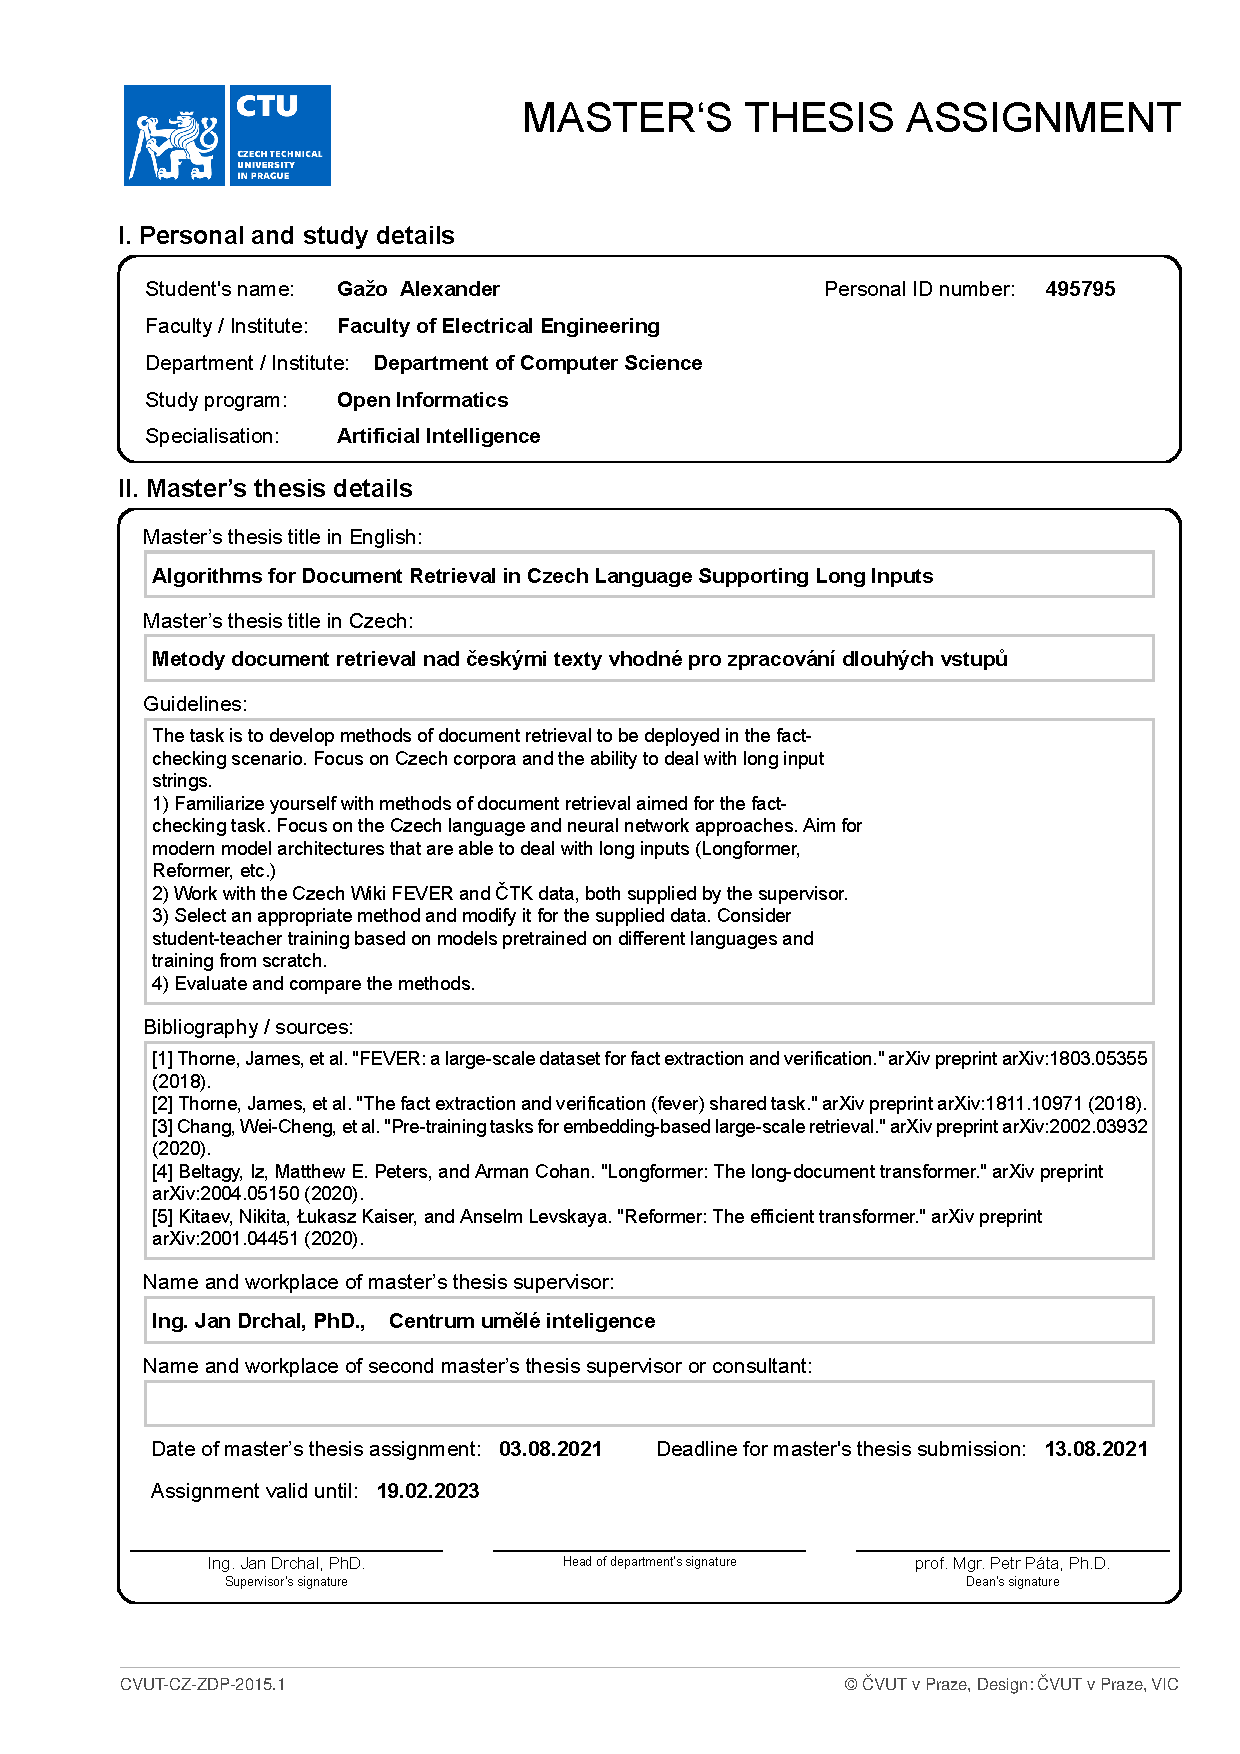
\includepdf[pages=-]{figures/assignment.pdf}
%%% Here should be a bound sheet included -- a signed copy of the "bachelor
%%% thesis assignment". This assignment is NOT a part of the electronic
%%% version of the thesis. DO NOT SCAN.

%%% A page with a solemn declaration to the bachelor thesis

\openright
\hypersetup{pageanchor=true}
\pagestyle{plain}
\pagenumbering{roman}
\vglue 0pt plus 1fill

\noindent
I declare that I carried out this master thesis independently and only with the cited
sources, literature, and other professional sources.

\medskip\noindent\sloppy
I understand that my work relates to the rights and obligations under Act No.~121/2000 Sb., the Copyright Act, as amended.
\vspace{10mm}

\hbox{\hbox to 0.5\hsize{%
In ........ date ............	% FIXME!
\hss}\hbox to 0.5\hsize{%
signature
\hss}}

\vspace{20mm}
\newpage

%%% Dedication

\openright

\noindent
\Dedication

\newpage

%%% Mandatory information page of the thesis

\openright

\vbox to 0.5\vsize{
\setlength\parindent{0mm}
\setlength\parskip{5mm}

Title:
\ThesisTitle

Author:
\ThesisAuthor

\DeptType:
\Department

Supervisor:
\Supervisor, \SupervisorsDepartment

Abstract:
\Abstract

Keywords:
\Keywords

\vss}

\vbox {
\begin{otherlanguage}{slovak}
\setlength\parindent{0mm}
\setlength\parskip{5mm}

Názov práce:
\ThesisTitleSk

Autor:
\ThesisAuthor

\DeptTypeSk:
\DepartmentSk

Vedúci bakalárskej práce:
\Supervisor, \SupervisorsDepartmentSk

Abstrakt:
\AbstractSk

Kľúčové slová:
\KeywordsSk

\end{otherlanguage}
\vss}

\newpage

\openright
\pagestyle{plain}
\pagenumbering{arabic}
\setcounter{page}{1}


%%% A page with the automatically generated table of contents of the bachelor thesis

\tableofcontents

%%% Each chapter is kept in a separate file
\chapter*{Introduction}
\addcontentsline{toc}{chapter}{Introduction}
\section*{Motivation}
At its early stages, the internet was envisioned to become the pinnacle of joint human effort to gather and easily retrieve expert knowledge on virtually any topic.
However, with many laypeople connected to the internet, extensive and aggressive advertising, and adversarial agents such as foreign powers or simply malicious individuals, the information on the internet is becoming harder to be trusted.
The information overload created by these agents results in an ``opaque'' state of the internet, where relevant and accurate information is hard to find in the mass of similarly sounding, non-professionally written sources.
Fact-checking the claims manually, therefore, becomes very expensive and time-consuming - bordering on unfeasible.
Nevertheless, multiple projects focused on fact-checking have emerged. 
Various platforms such as Instagram\footnote{\url{https://about.fb.com/news/2018/05/hard-questions-false-news/}} and Twitter\footnote{\url{https://blog.twitter.com/en_us/topics/product/2021/introducing-birdwatch-a-community-based-approach-to-misinformation}} have incorporated fact-checking mechanisms, mainly on viral post and posts of politicians. 

In Czechia and the Slovak Republic, a popular project is Demagog\footnote{\url{https://demagog.cz}}, whose goal is to verify politicians' claims.
The claim verification is carried out manually using primary sources. 
Similar foreign projects are PolitiFact\footnote{\url{https://www.politifact.com/}}, Factcheck.org\footnote{\url{https://www.factcheck.org/}}, and Washington Post Fact Checker\footnote{\url{https://www.washingtonpost.com/news/fact-checker/}}.
Multiple past "public debates", such as the European migrant crisis or the current coronavirus pandemic, have highlighted the need for such systems since there is a need for accurate and up-to-date information.
The process is very labor-intensive, and thus, there is a natural demand for automatization.

The recent advances in natural language understanding, mainly the introduction of transformer architecture \citep{attention-is-all-you-need} and the BERT model \citep{bert}, led to new research on the use of neural methods in fact-checking.
The FEVER\footnote{\url{https://fever.ai/}} paper \citep{fever} has led this effort since 2018, focusing on creating a dataset meant for training neural models.
They succeeded in creating a sizeable human-annotated dataset and were able to train a pipeline model on it.
The model first retrieved relevant documents (the document retrieval task) and then labeled the initial claim based on these documents. 
%Since then, the FEVER team held multiple shared tasks, and the pipeline approach proved to be adequate.
With better models released every year, the long-term goal is to create a model capable of correctly assessing a claim's truthfulness and provide satisfactory evidence. However, creating helpful tools for journalists to assist them in the fact-checking scenario is the goal for now.

On the other hand, the advances also provide new ways of creating false information on a large scale. Such an example is the recently introduced GPT-3 model \citep{gpt}, which is able to generate human-sounding English texts.
The potential ability of adversaries to flood the internet with fake news articles emphasizes the need for scalable fact-checking tools.

Automatic fact-checking should not be thought of as the miracle cure to the fake news problem, which is much more complex and deserves a society-wide approach.

\section*{AI in Journalism}

This thesis is one of the multiple theses written by the fact-checking team at ČVUT, led by Ing. Jan Drchal, Ph.D., as part of the AI in Journalism project, supported by the Transformation of Journalisms Ethics in the Advent of Artificial Intelligence (TL02000288)\footnote{\url{https://starfos.tacr.cz/cs/project/TL02000288}} grant from the Technology Agency of the Czech Republic.
Our team focuses on creating a Czech fact-checking dataset from the ground up, and developing usable Czech models for the fact-checking task, inspired by FEVER \citep{fever} and \citet{danish_fever}.
The dataset is based on Czech news articles provided in cooperation with the Czech News Agency\footnote{Česká Tlačová Agentúra (ČTK)} -- we refer to the completed dataset as the ČTK dataset. 
Our colleague \citet{ullrich} describes the creation of the ČTK dataset, which consisted of building a Czech annotation platform, working with annotators (students of the Faculty of Social Sciences at Charles University, one of our partners), and analyzing and cleaning up the gathered data.
The works from colleagues \citet{dedkova} and \citet{rypar} deal with various aspects of document retrieval -- the use of hybrid (multi-stage) models and the performance of different embedding paradigms, respectively.

\section*{Transformer Models}

The original transformer architecture \citep{attention-is-all-you-need} and BERT-model \citep{bert} are based on feeding fully-connected feed-forward networks with token representations aggregated from the whole text, meaning that the information from the input tokens (words or subwords) is adjusted according to their whole context. 
This mechanism, named ``attention'' by the authors \citep{first-attention}, introduces quadratic time complexity by ``attending'' to all the input tokens for each input token.
The input of BERT is thus usually limited to 512 tokens as a design choice.
Working with this restriction, we decided to split the \CTK{} articles into paragraphs and perform document retrieval on them, theoretically losing joint article meaning.

In this thesis, we study this practice and compare it to working with full articles using BERT-based models with altered attention mechanisms such as \nystr{} \citep{nystrom}, Longformer \citep{longformer} and Reformer \citep{reformer}.
The changes allow for longer inputs without increasing the computation cost, compromising in other areas.

\section*{Thesis Outline}

This thesis focuses on the document retrieval part of the fact-checking pipeline.
Specifically, it deals with models suitable for processing long Czech documents.

The first chapter deals with fact-checking as a formal task and the past advances in this field.
The next chapter formally defines document retrieval and introduces traditional as well as novel approaches. 
% The datasets created in the project are described in the third chapter, where t
% In Chapter \ref{chap:docret}, we formally define document retrieval, introduce methods that are already in use, and methods that we will be exploring further in this thesis. 
The FEVER dataset, its Czech-translated version, and the ČTK dataset are in-depth described in the third chapter.
We also analyze the length of the documents upon which the datasets are built.
% The before-mentioned datasets are in-depth described in the next chapter (Chapter \ref{chap:data}).
We dedicate the last two chapters to the proposed solutions and the results of the evaluation.

\chapter{Document Retrieval}
\label{chap:docret}

The term document retrieval refers to the task of finding relevant information to user queries in a large set of records (documents). 
% Therefore, the document retrieval system operates over a database of records, which for this thesis are described in \ref{chap:data}.
One can think of document retrieval as a search in a vast database of documents. 
In this view, web search services, such as Google, are a form of document retrieval. The database of documents are all accessible web pages on the internet, and the user query functions as the search query.

For our uses, the query is the claim to be fact-checked, and the document database is a collection of relevant documents, which we call knowledge scope. 

\section{Formal Description}
The task can be formally described \citep{two-tower} using a scoring function (sometimes referred to as ranking function) %article before ranking maybe
$$f\colon\mathcal{D}\times\mathcal{Q}\rightarrow\R$$
that maps a document-query pair $(d, q)$ to a score $f(d,q)$. 
Then, typically, the documents in pairs with the highest scores are considered to be the proposed solution to the task. 

This definition also fits a description of a range of other tasks such as open-domain question answering \citep{wiki-retrieval} or recommendation systems.

\section{Approaches to Document Retrieval}
% TODO two tower paper, 
In order to solve the document retrieval task, we will focus on finding an appropriate function $f$.
In this thesis, that means a function suitable for long documents.

This thesis explores both neural and non-neural (traditional) approaches to designing the scoring function, with emphasis on the neural approach while using the other as the baseline.

% This section introduces the most common methods of document retrieval, as well as new models with great potential.

\subsection{Traditional Approaches}

\subsubsection{TFIDF}

The traditional approaches are motivated by the intuition that relevant documents will contain the same words as those present in the query. 
Longer documents are at an advantage since there is a higher chance of the relevant words being present, so the term count is often normalized by the number of all terms in the document.
This simple metric is called term frequency (TF). 

TF can be ineffective if some of the terms in the query are very common in the document database.
This issue is resolved by introducing inverse document frequency, which informs how common the term is across all the documents.
The base version of IDF:
$$\text{idf}(t, D)=\log{\frac{\abs{D}}{\abs{\{d\in D: t\in d\}}}}\ .$$

% If we combine these two metrics
Multiplying these two metrics, we get the TFIDF weight of term $t$ in document $d$ in document database $D$:
%which is calculated simply as
$$\text{tfidf}(t,d,D)=\text{tf}(t,d)\cdot\text{idf}(t,D)\ .$$

We have explained how to compute each term's weight ("importance") in each document.
The intuitive formula for query score $f(q, d)$ is then
$$
f_D(q, d)\sim\sum_{t \in q}\text{tfidf}(t, d, D)\ .
$$
% TFIDF is called weighting scheme exactly for this reason. % toto urcite inam

This formula can be improved -- in this form, it favors longer queries $q$.
We can also precompute the TFIDF values for each document and vocabulary word in the corpus.
Thus we obtain $|D|\times {vocabulary\_size}$ matrix $V$ of TFIDF values.
To get the relevance of each document to the query $q$, that is $f_D(q, d)$, we first represent the query $q$ as a bag of words vector, corresponding to the columns of our precomputed TFIDF matrix $V$, ignoring words that appear in the query only. %only in the query?
The resulting score is then the normalized (not to favor long queries or documents) dot product of a row of the matrix and the BOW representation of the query $q$, denoted $\vec{q}$.
We can obtain the scores for every query document pair by matrix multiplication:
$$
f_D(q, d) = \frac{V\vec{q}}{|\vec{q}|} \in \R^{|D|}\ ,
$$
provided that matrix $V$ is row-normalized (euclidian norm of each row is equal to one).
Please note that this is equivalent to computing the cosine similarity for each document and query vector pair.

This function is one of the first and still widely used \citep{Beel2016} metrics for document retrieval. 

Some of the apparent disadvantages of TFIDF are the lack of semantic meaning that comes from the independence on the word order and matching exact words only. % independence???
The former may be improved by using n-grams and the latter using character level features, which is especially helpful in inflected languages such as Czech.
On the other hand, TFIDF is, to this day, a very well-performing low-computation cost ranking function.

Over the years, multiple versions of the TFIDF approach appeared, differing slightly in formulas or weights of the factors. One of such versions is Best Match 25.
% maybe put the last sentence as the last sentence of the whole section

\subsubsection{Best Match 25 (BM25)}

One of the best performing versions \citep{bm_vs_tfidf} is Best Match 25 (BM25) by \cite{bm25}.
The original formula is:
$$
\text{BM25}(q, d) = 
        \log \text{idf}(t, d)
        \cdot \frac{(k_1 + tf_{t, d})}{k_1((1-b) + b \cdot (L_d / L_{avg})) + tf_{t, d}} 
        \cdot \frac{(k_3 + 1)tf_{t, q}}{k_3 + tf_{t, q}}.
$$

The commonly used formula is
$$
\text{BM25}(Q,D)=\sum^n_{i=1}\text{IDF}(q_i)\frac{f(q_i, D)(k_1+1)}{f(q_i,D)+k_1\left(1-b+b\frac{\abs{D}}{\text{avdgl}}\right)}
\ ,$$
which differs from the original formula in several parameters (initially, four) due to setting these parameters to neutral values.

In the formula, $Q$ is a query consisting of words $q_1,\ldots,q_n$, $f(q_i,D)$ is a frequency of keyword $q_i$ in the document $D$, $|D|$ is a length of the document $D$. 

%TODO problem with long documents - BM25+ http://sifaka.cs.uiuc.edu/~ylv2/pub/cikm11-lowerbound.pdf

This approach does not account for word variations and the real meaning.
However, it, to this day, represents a solid baseline as reported by \cite{weak_baselines}.

\subsection{Neural Approaches}

When dealing with natural language processing, we can approach the task in two different ways, both described in detail by \cite{two-tower}. 

The first is to have the document-query pair $(d,q)$ on the input of the neural model (cross-attention model).
One of the benefits is the direct usage of the neural model on the downstream tasks, possibly granting better performance.

The second approach is to preprocess the whole database of documents by the model and then using some metric for choosing the documents related to the query based on the computed representation.
The obvious advantage is the offline preprocessing and thus improved performance during inference.
Only the unseen query has to be processed by the neural model followed by computing the metric between the documents' representation and the query representation.
This is usually way faster than using a neural model for every document and can also be significantly spedup \citep{faiss}.
The obvious disadvantage is the need for additional space to store the precomputed representation.

We will be using the second approach as our computational resources are limited.

% TODO under this line ---------------------------------
\subsubsection{BERT}
In 2018, BERT \citep{bert} the now well-established NLP model was introduced. The model is pre-trained using the masked language modeling task and the next sentence prediction task.
The defining feature of BERT is its self-attention mechanism, which attends to the whole input at once and transforms input tokens based on full context, both left, and right to the token.
Since the "each versus each" approach is employed, this mechanism naturally introduces $O(N^2)$ time complexity, which acts as a bottleneck in applications, where a longer input is required.
Since its introduction, there have been many well-performing models based on BERT (this movement is sometimes referred to as "BERTology").
In this thesis, we will focus on models which use similar architecture and modify attention mechanism in order to be able to compute long inputs.
% used usually for GLUE benchmark which is not???? for document retrieval
% TODO maybe include attention formula

\subsubsection{Longformer}

Longformer model \citep{longformer} arises when instead of computing the whole $QK^T$, only certain regions (usually specific diagonals) are calculated, thus reducing the model time complexity allowing for longer inputs.
Huggingface models are available.

\subsubsection{Reformer}

Reformer model \citep{reformer} offers two improvements to the transformer model.
The first is the usage of locality-sensitive hashing in the attention mechanism, which in order to approximate the full attention matrix focuses for each input token only on the closest tokens.
The closest tokens are found using the locality-sensitive hashing function.
This, coupled with memory saving features, offers a model which can have a whole novel as its single input.

\subsubsection{Performer}

Performer model \citep{performer} looks at the self-attention mechanism as a kernel function and introduces randomized feature functions such that the expected value of scalar product %????%e
of the resulting feature vectors is equal to the true value.
% TODO weak ensurences

\subsubsection{Nyostromformer}

Nyostromformer \citep{nystrom} uses "smart" Moore-Penrose inverse approximation. Instead of full $Q$ and $K$ matrices, only segment-means are used, and then the Moore-Penrose inverse is calculated using an iterative algorithm.

\subsubsection{ColBERT}



\chapter{Datasets}
\label{chap:data}

% TODO was it really mentioned
As mentioned, the primary dataset, usage-wise and inspiration-wise, was the FEVER dataset \citep{fever}.
Deriving \cite{fever} methods, we \citep{ullrich} were able to create our own FEVER-like database using Czech News Agency's infobank, to which we had the access granted thanks to the GAČR grant.  

\section{FEVER}

Fact Extraction and Verification \citep{fever} dataset is a large-scale dataset based on Wikipedia articles.
The dataset was created by extracting sentences from English Wikipedia articles and classifying them by human annotators as Supported, Refuted, or NotEnoughInfo.
The evidence, either single or multiple articles or even paragraphs proving or disproving the claim, is also recorded.
The complete FEVER contains 185,445 annotated claims generated using 50,000 popular articles.

The creation consisted of two steps. The sentences were manually extracted from popular Wikipedia articles.
Then, to create a more diverse set of claims, the annotators had the option of producing new claims by mutating the existing ones in various ways (generalizing, specification, entity substitution, non-trivial negating, and rephrasing).
More complex claims were created by providing hyperlinked Wikipedia articles as another source of information while mutating the claim.
In the second step - annotation - the annotators were asked to label the generated claims and provide suggested evidence when needed.
The whole process was streamlined in order not to spend longer than five minutes on a single claim throughout all stages.

The quality of the dataset was throughoutly tested in the paper.
One of the methods was the fact that each generated claim was annotated multiple times to prevent mislabeling.

\section{ČTK}
% nomenclature

Thanks to the GAČR grant, we were granted access to the Czech News Agency's infobank. 
Inspired by \cite{fever} and \cite{danish_fever}, our colleague \cite{ullrich} created a czech version of the claim extracting and labeling software tool running over the ČTK infobank's articles. 
It was prepared to be used by layman annotators, who were students of our grant partner - the Faculty of Social Sciences at Charles University.
%In the cooperation with Faculty of Social Sciences, we were able to create 
%Annotators were provided in cooperation with the Faculty of Social Sciences.

%TODO GACR grant a sucasti

The dataset creation consisted of two harvests. 
After reviewing the results of the first one, we were able to rewrite instructions in the tool to guide the annotators to create higher-quality mutations and labels with fewer conflicts.
The second harvest concluded with $\circ$ 3,500 labeled claims, with more than half of them being labeled two or more times. %TODO cite webpage
As of writing, this figure is not final as the dataset needs to be manually cleaned and have conflicts resolved. 


\chapter*{Conclusion}
\addcontentsline{toc}{chapter}{Conclusion}

We introduced the problem of fact-checking and described modern approaches to the problem.
We explained the motivation for studying the topic and proposed using new neural models to help with automatic fact-checking.
Our research team created the first fact-checking dataset in the Czech language \citep{ullrich} and explored different models' architectures capable of good performance.
Inspired by the FEVER pipeline \citep{fever} (see Figure \ref{fig:pipeline}), we split the problem into two distinct tasks -- document retrieval and natural language inference.

In this thesis, we deal with the document retrieval task.
We first defined the task formally and then introduced well-established traditional techniques for the task.
Then followed a brief description of the progress from RNN-based language models to transformers \citep{attention-is-all-you-need} and BERT \citep{bert}.
Since the BERT model as described in \citep{bert} and as adopted across the research field perform best only for inputs up to 512 tokens, we were forced to work over paragraphs instead of the whole documents. 
Our colleagues \citep{rypar} and \citep{dedkova} studied this type of document retrieval.

This thesis explored whether we could improve retrieval performance by utilizing whole articles. 
We provided a summary of currently available papers regarding transformer language models supporting long inputs, namely Longformer, BigBird, Reformer, Linformer, Performer, and \nystr{}.
Since no pre-trained models for the Czech language were available, we either trained them from scratch or utilized the student-teacher method \citep{student-teacher} described in Section \ref{subsec:distillation}.
Lastly, we compared the traditional, short-input, and long-input approaches in the document retrieval task and analyzed the results.

The resulting models turned out not to outperform classic BERT with paragraph-level splitting, but TODO.

\subsubsection{Future Work}

As time progresses, automatic fact-checking will be needed more and more.
With the joint effort across the machine learning research field, we hope to train better TODO.
We wish to continue improving the created \CTK{} dataset and to now focus on the natural language inference task of the fact-checking pipeline. 

%%% Bibliography
%%% Bibliography (literature used as a source)
%%%
%%% We employ bibTeX to construct the bibliography. It processes
%%% citations in the text (e.g., the \cite{...} macro) and looks up
%%% relevant entries in the bibliography.bib file.
%%%
%%% The \bibliographystyle command selects, which style will be used
%%% for references from the text. The argument in curly brackets is
%%% the name of the corresponding style file (*.bst). Both styles
%%% mentioned in this template are included in LaTeX distributions.

\bibliographystyle{plainnat}    %% Author (year)
% \bibliographystyle{unsrt}     %% [number]

\renewcommand{\bibname}{Bibliography}

%%% Generate the bibliography. Beware that if you cited no works,
%%% the empty list will be omitted completely.

\bibliography{bibliography}

%%% If case you prefer to write the bibliography manually (without bibTeX),
%%% you can use the following. Please follow the ISO 690 standard and
%%% citation conventions of your field of research.

% \begin{thebibliography}{99}
%
% \bibitem{lamport94}
%   {\sc Lamport,} Leslie.
%   \emph{\LaTeX: A Document Preparation System}.
%   2nd edition.
%   Massachusetts: Addison Wesley, 1994.
%   ISBN 0-201-52983-1.
%
% \end{thebibliography}


%%% Abbreviations used in the thesis, if any, including their explanation
%%% In mathematical theses, it could be better to move the list of abbreviations to the beginning of the thesis.
%\chapwithtoc{List of Abbreviations}

\openright
\end{document}